\fancyfoot[C]{Kronberger}

%% Human-Computer Interaction System %%%%%%%%%%%%%%%%%%%%%%%

\chapter{Human-Computer Interaction System}

\section{Übersicht}
Das Human-Computer Interaction System ist, wie der Name schon verrät, die Komponente, welche als Schnittstelle zwischen dem Nutzer und dem gesamten elektrischen System dient. Durch es sollte die fehlerfreie Nutzung der Funktionen des Motorrades gewährleistet sein, ebenso sollte es wichtige Fahrdaten und andere Informationen speichern und dem User anzeigen können.\\
Wichtig ist das System, troz der großen Komplexität, so intuitiv und nutzerfreundlich wie möglich zu gestallten.

\subsection{Grundfunktionen des Systems}
Die geplanten Funktionen des HCIS lassen sich grob in vier Grundfunktionen einteilen.
\begin{itemize}
	\item \textbf{Steuerung der Peripherie} \medskip\\
	Die Schalter und Buttons am Lenker, welche zuvor über den Kabelbaum die Leuchten, Blinker oder der Hupe gesteuert haben. Werden nun über die General-purpose input/output (GPIO) anschlüsse des Raspberry Pi Micro Computers gesteuert.
	\item \textbf{Graphische Benutzeroberfäche}\medskip\\
Dient der Anzeige wichtiger Fahr- und Ladedaten welche entweder in echtzeit oder über die Datenbankschnittstelle abgerufen und graphish angezeigt werden können.
	\item \textbf{Kommunikation mit den Steuereinheiten des Motorrades} \medskip\\
	Über CAN-Bus werden Daten von dem Batterie Management Systems (BMS) und der Curtis Motorsteuerung empfangen und an die Benutzeroberfläche zur echtzeit verwertung und an die Datenbankschnittstelle zur Langzeitsicherung der Fahrdaten weiter gegeben.
	\item \textbf{Speichern der relevanten Fahrdaten über die Datenbankschnittstelle} \medskip\\
Die über den CAN-Bus empfangenen Daten werden sofort an die Datenbankschnittstelle (Hander) weitergegeben um für Datenauswertung und Testberichte die Daten zu speichern. Ebenso bezieht das Diagnosesystem der Benutzeroberfläche die Daten über diese Schnittstelle.
\end{itemize}
\newpage

\subsection{Grundaufbau des Systems}
In der Abbildung wird der Grundaufbau des Systems und die Datenverbindungen der folgenden  Komponenten veranschaulicht.

\begin{itemize}
	\item Raspberry Pi - Die Steuereinheit des Systems.
	\\ Kommuniziert über CAN-Bus mit den anderen Steuerkomponenten des Motorrades.
	\item User Input - Die vorhandenen Buttons am Lenker des Motorrads werden über pull down Widerstände mit den Inputs des Raspberry Pi verbunden. 
	\item Peripherie - Die Grundkomponenten des Motorrades wie Scheinwerfer oder Hupe.
	\item Dashboard - Der Bildschirm zur Anzeige der Verarbeiteten Informationen.
\end{itemize}

\begin{figure}[H]
	\begin{center}
		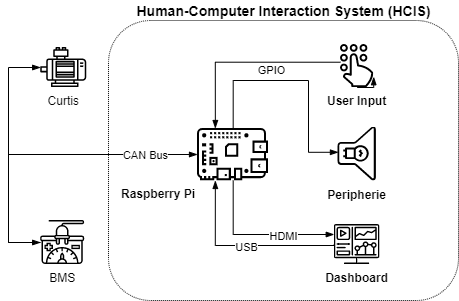
\includegraphics[scale=0.5]{figures/hcis/HCIS_Grundfunktion.png}
		\caption{Grundaufbau des Human-Computer Interaction Systems}
	\end{center}
\end{figure}

Nicht in der Abbildung dargstellt ist die Versorgung der einzelnen Komponenten, welche in dem folgenden Abschnitt noch genauer erläutert wird.

\newpage

%% Versorgung %%%%%%%%%%%%%%%%%%%%%%%%%%%%%%%%%%%%%%%%%%%%%%% 

\section{Versorgung}
\subsection{Aufbau des Versorgungssystems}
\subsection{Spannungswandler}
\subsubsection{5V Versorgungssystem}
\subsubsection{12V Versorgungsysstem}

\newpage

%% Steuerung der Peripherie %%%%%%%%%%%%%%%%%%%%%%%%%%%%%%%%%

\section{Steuerung der Peripherie}
\subsection{Hardware}
\subsubsection{Input}
\subsubsection{Output}

\subsection{Software}
\subsubsection{GPIO Zero}
\subsubsection{Threading}

\newpage

%% Benutzeroberfläche %%%%%%%%%%%%%%%%%%%%%%%%%%%%%%%%%%%%%%%

\section{Benutzeroberfläche}

\subsection{Pages}
\subsection{Implementierung der Benutzeroberfäche}
\subsubsection{QML}
\subsubsection{Qt-Quick}
\subsubsection{Slots and Signals}
Slots und Signals werden in Qml zur ereignisgesteuerte Kommunikation zwischen front-end und back-end verwendet. In der folgenden Illustration wird diese anhang eines einfachen Beispiels erklärt.
\begin{center}
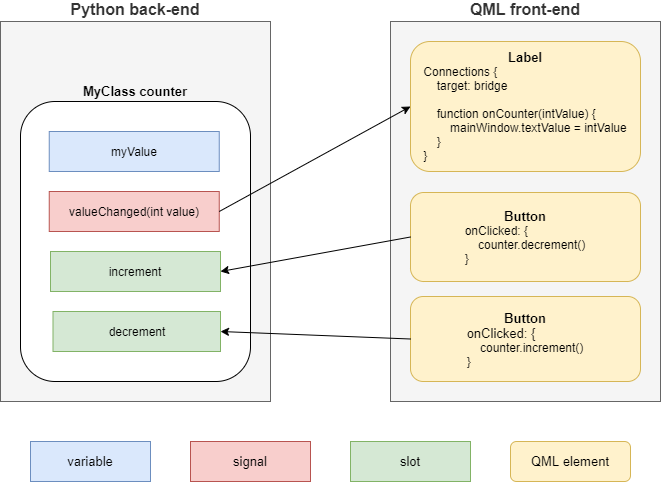
\includegraphics[scale=0.5]{figures/hcis/signals_slots.png}
\end{center}

\textbf{Signals}\\ \medskip
	Diese können als "Mitteilungen" angesen werden welche über das Aufrufen der signal.emit funktion vom back-end an das front-end gesehendet wird. Im front-end wird wiederum eine eigens definierte Funktion benötigt um dem Wert einem Property eines QML Elements zuzuweisen.
	\item \textbf{Slots}\\ \medskip
	Slots sind Call-Back funktionen. 
	
\subsubsection{Bridge}

\newpage

%% Kommunikation %%%%%%%%%%%%%%%%%%%%%%%%%%%%%%%%%%%%%%%%%%%%

\section{Kommunikation}
\subsection{Hardware}
\subsection{Listener}
\subsubsection{Receive Data}

\newpage

%% Fahrdatenspeicher %%%%%%%%%%%%%%%%%%%%%%%%%%%%%%%%%%%%%%%%

\section{Fahrdatenspeicher}
\subsection{Datenbankstruktur}
\subsubsection{Login System}
\subsubsection{Motor Daten}
\subsubsection{Akku Daten}
\subsection{Handler}
\subsubsection{SELECT Befehl}
\subsubsection{INSERT Befehl}

\newpage